\chapter{Environment Description}
\label{cha:env_description}
\lipsum \autocite{DBLP:books/sp/HarderR01}



\section{arena description}


This section describes the simulated environment and agent in detail. The environment is a 3D simulation of a physical arena at the ScaDS.AI research facility. The simulated arena consists of a rectangular platform with enclosing walls. Simulated light sources illuminate the platform from above.
The goal of our agent is to complete tracks in the arena by traversing the track's goals in order. Each goal consists of 2 cuboid pillars of the same colour. The pillars are coloured red or blue. The goals' colours alternate in the track. The distance between the pillars is fixed and the same for all goals. The positions of the goals depends on the episode's track. The tracks are grouped by the difficulty settings easy, medium and hard. 

The tracks in the easy setting contain 3 goals that are positioned on the arena's center line with even distances between them. The medium setting contains 3 goals that are shifted on the center line towards the arena's walls. The hard setting contains 3 goals that are shifted on the center line towards the arena's walls, resulting in a zig-zag pattern. The zig-zag pattern is the most challenging for the agent to navigate, as it requires the agent to turn sharply to pass the goals. One track from each difficulty setting is shown in figure \ref{fig:track_difficulty_settings}. The tracks in each setting are structurally very similar to each other. They differ in goal coloring and the orientation of the shift from the center line.


\begin{figure}
    \centering
    \subfigure[Easy]{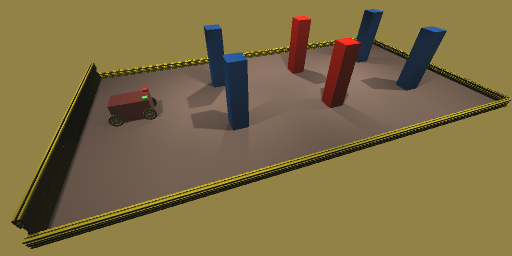
\includegraphics[width=0.3\textwidth]{Bilder/evaluation_easy.png}}\qquad
    \subfigure[Medium]{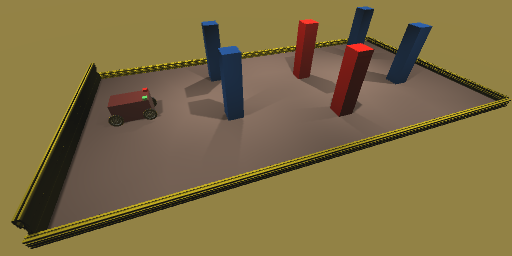
\includegraphics[width=0.3\textwidth]{Bilder/evaluation_medium.png}}\qquad
    \subfigure[Hard]{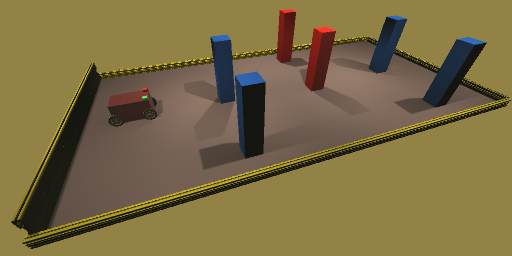
\includegraphics[width=0.3\textwidth]{Bilder/evaluation_hard.png}}\\
    \caption{Example evaluation tracks for each difficulty setting.}
    \label{fig:track_difficulty_settings}
\end{figure}
% the images are generated with image_printer.py


There are three light settings for the environment, bright, standard and dark. The different light settings are achieved by varying the light intensities of the light sources above the arena and changing the horizon in the agent's camera.

\begin{figure}
    \centering
    \subfigure[Arena Bright]{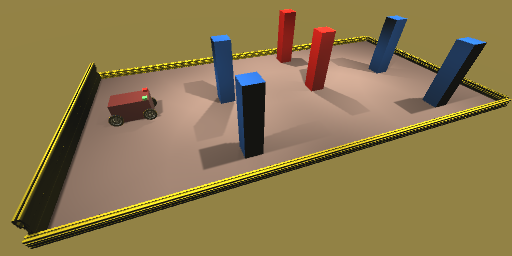
\includegraphics[width=0.3\textwidth]{Bilder/light_setting_bright_arena.png}}\qquad
    \subfigure[Arena Standard]{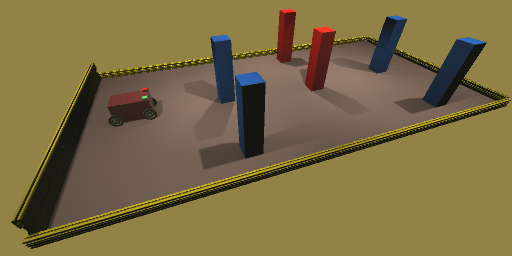
\includegraphics[width=0.3\textwidth]{Bilder/light_setting_standard_arena.png}}\qquad
    \subfigure[Arena Dark]{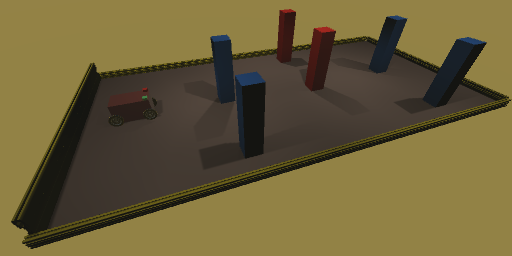
\includegraphics[width=0.3\textwidth]{Bilder/light_setting_dark_arena.png}}\\
    \subfigure[Agent Bright]{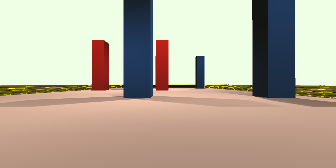
\includegraphics[width=0.3\textwidth]{Bilder/light_setting_bright_pov_no_preprocessing.png}}\qquad
    \subfigure[Agent Standard]{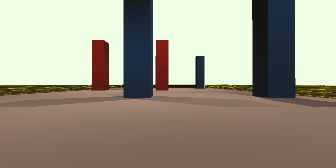
\includegraphics[width=0.3\textwidth]{Bilder/light_setting_standard_pov_no_preprocessing.png}}\qquad
    \subfigure[Agent Dark]{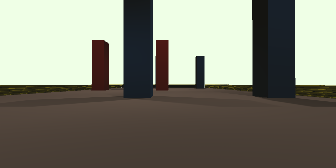
\includegraphics[width=0.3\textwidth]{Bilder/light_setting_dark_pov_no_preprocessing.png}}\\
    \caption{Arena and agent camera under different light settings.}
    \label{fig:track_light_settings}
\end{figure}
%light_setting_{name}_arena.png
%light_setting_{name}_pov_no_preprocessing.png

% TODO sieht die grafik gut aus?






\section{Agent Description}

The agent is modeled after the NVIDIA JetBot, a small robot designed for educational purposes. The NVIDIA JetBot is equipped with a camera and a differential drive system. The agent's camera is mounted on the JetBot's front and captures the arena from the JetBot's perspective. The camera captures the arena in a 2D image format. 
There are two versions of the JetBot agent in the simulation, the DifferentialJetBot and the FourWheelJetBot. The DifferentialJetBot has two driving wheels at the front and a ball supporting it at the back. The FourWheelJetBot has 2 steering driving wheels at the front and two non-driving wheels in the back. The DifferentialJetBot steers by applying different torques to the two front wheels. The FourWheelJetBot steers by turning the front wheels in the desired direction and applyig equal torques to both wheels.
The FourWheelJetBot was used in the work by \autocite{maximilian}. The DifferentialJetBot was developed to match the physical NVIDIA JetBot more closely. The two JetBot designs are shown in figure \ref{fig:jetbots}.

\begin{figure}
    \centering
    \subfigure[Nvidia JetBot Photo]{\includegraphics[width=0.3\textwidth]{Bilder/nvidia_jetBot.png}}\qquad
    \subfigure[DifferentialJetBot]{\includegraphics[width=0.3\textwidth]{Bilder/differential_jetBot.png}}\qquad
    \subfigure[FourWheelJetBot]{\includegraphics[width=0.3\textwidth]{Bilder/fourwheel_JetBot.png}}\qquad
    \caption{Original Nvidia JetBot and simulated JetBot Desgins}
    \label{fig:jetbots}
\end{figure}


\section{Episode Design}

time-limit, episode termination, step-function, Collisions, rewards

time limit explain here

\label{time_limit}
% TODO describe the timelimit in env description
